\section{Dreiphasenwechselstrom (Drehstrom)}
	%\subsection{Entstehung des Drehstrom-Systems}
		\begin{tabular}{p{8.5cm}p{9cm}}
        	\begin{minipage}{8cm}
            	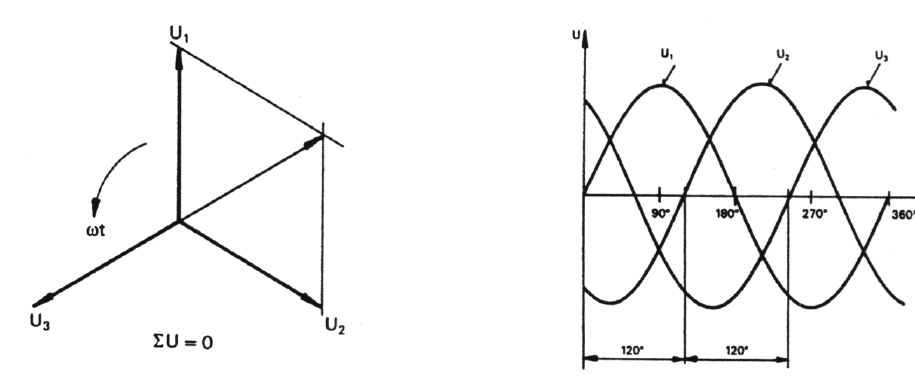
\includegraphics[width=7.5cm]{bilder/Drehstrom.png}
            \end{minipage} &    
			\begin{minipage}{10cm}
            	Zeiger drehen mit $\omega t$ im Gegenuhrzeigersinn ($\omega > 0$). \\
            	$\underline{U}_2$ ist gegenüber $\underline{U}_1$ 
				$120^{\circ}$ nacheilend, $\underline{U}_3$ gegenüber $\underline{U}_1$ $240^{\circ}$.  \\ \\
				Somit gilt (bei symmetrischer Belastung): \\
				$\underline{U}_2 = \underline{U}_1 \cdot e^{j (-120^{\circ})}; \underline{U}_3
				= \underline{U}_1 \cdot e^{j (-240^{\circ})} = \underline{U}_1 \cdot e^{j
				(120^{\circ})}$
            \end{minipage}
        \end{tabular}
		
% 		\subsubsection{Verketten der Spannungen oder Str\"ome}
% 			\begin{tabular}{p{5cm}p{6cm}p{7cm}}
%             	\textbf{Maschensatz} &
%             		\fbox{$\underline{U}_1 + \underline{U}_2 + \underline{U}_3 = 0$} \\
%             	\textbf{Knotenpunktsatz} &
%             		\fbox{$\underline{I}_1 + \underline{I}_2 + \underline{I}_3 = 0$} \\
%             \end{tabular}

		\subsubsection{Stern- (Y) / Dreieckschaltung ($\Delta$)}
            	\renewcommand{\arraystretch}{1.5}
			\begin{tabular}{| p{4.5cm} | l | l |}
				\hline
	 				& Sternschaltung (Y)		& Dreieckschaltung ($\Delta$)\\
	 			\hline
	 			\vspace{0.2cm}
	 				%\textbf{Zeigerdiagramm} & & \\ 
	 				&
	 					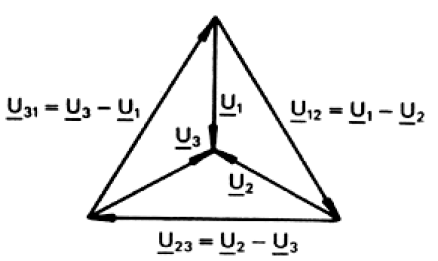
\includegraphics[width=5cm]{bilder/Sternspannung.png} &
	 					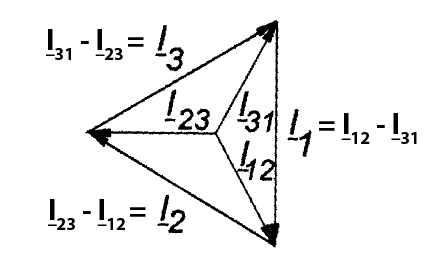
\includegraphics[width=5cm]{bilder/Dreieckstrom.png} \\
						
					Phasenverschiebung &
						$U_1 = 400V; U_2 = 400Ve^{-j120^\circ}; U_3 = 400Ve^{j120^\circ}$&
						\\
		 			Verkettete Spannung &
		 				$U = U_{Str} \cdot \sqrt{3}$ \hspace{0.2cm} $\underline{U} = \underline{U}_{Str} \cdot \sqrt{3} \cdot e^{j 30^\circ}$ &
		 				$U = U_{Str}$ \hspace{0.2cm} $\underline{U} = \underline{U}_{Str}$ \\
		 			Aussenleiterstr\"ome &
		 				$I = I_{Str}$ \hspace{0.2cm} $\underline{I} = \underline{I}_{Str}$ &
		 				$I = I_{Str} \cdot \sqrt{3} $ \hspace{0.2cm} $\underline{I} =
		 				\underline{I}_{Str} \cdot \sqrt{3} \cdot e^{-j 30^\circ} $ \\ Gesamt-Scheinleistung &
		 				$S = 3 \cdot S_{Str} =\sqrt{3} \cdot U \cdot I $ \hspace{0.2cm} in $[VA]$
		 				& $S = 3 \cdot S_{Str} = \sqrt{3} \cdot U \cdot I$ \hspace{0.2cm} in $[VA]$ \\ Scheinleistung pro Strang &
		 				\multicolumn{2}{l|}{\hspace{3cm} $S_{Str} = U_{Str} \cdot I_{Str}$ \hspace{0.2cm} in $[VA]$} \\
		 			Wirkleistung &
		 				\multicolumn{2}{l|}{\hspace{3cm} $P = S \cdot \cos\varphi = \sqrt{3} \cdot U \cdot I \cdot \cos\varphi$ \hspace{0.2cm} in $[W]$} \\
		 			Blindleistung &
		 				\multicolumn{2}{l|}{\hspace{3cm} $Q = S \cdot \sin\varphi = \sqrt{3} \cdot U \cdot I \cdot \sin\varphi$ \hspace{0.2cm} in $[var]$} \\
% 		 			Wirkarbeit &
% 		 				\multicolumn{2}{l|}{\hspace{3cm} $W = P \cdot t = \sqrt{3} \cdot U \cdot I \cdot cos\varphi \cdot t$ \hspace{0.2cm} in $[Ws, kWh]$} \\
% 		 				&\multicolumn{2}{c|}{}\\
% 		 			Blindarbeit &
% 		 				\multicolumn{2}{l|}{\hspace{3cm} $W_b = Q \cdot t = \sqrt{3} \cdot U \cdot I \cdot sin\varphi \cdot t$ \hspace{0.2cm} in $[varh, kvarh]$} \\
	 			\hline
			\end{tabular}
        \renewcommand{\arraystretch}{1}
		
		%\subsubsection{Bestimmung des Y-Punktes mittels Leitwert-Operatoren im Vierleiter-Drehstromnetz}
        \subsubsection{Ausfall des Neutralleiters: Bestimmung des Y-Punktes mittels Leitwert-Operatoren}
            \begin{tabular}{p{5cm}p{13cm}}
            	\begin{minipage}{8cm}
                	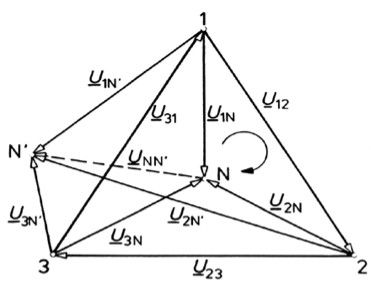
\includegraphics[width=5cm]{bilder/ZeigerdarstellungVerschobenerSternpunkt.png}
                \end{minipage} &
				\begin{minipage}{13cm}
                	$\underline{U}_{12} = \underline{U}_{1N'} - \underline{U}_{2N'}$ \hspace{0.3cm}
                	$\underline{U}_{1N'} = \underline{U}_{1N} + \underline{U}_{NN'}$ \hspace{0.3cm}
                	$\underline{I}_1 = \underline{Y}_1 \cdot \underline{U}_{1N'} = \underline{Y}_1 \cdot (\underline{U}_{1N} + \underline{U}_{NN'})$ \\
                	$\underline{U}_{23} = \underline{U}_{2N'} - \underline{U}_{3N'}$ \hspace{0.3cm}
                	$\underline{U}_{2N'} = \underline{U}_{2N} + \underline{U}_{NN'}$ \hspace{0.3cm}
                	$\underline{I}_2 = \underline{Y}_2 \cdot \underline{U}_{2N'} = \underline{Y}_2
                	\cdot (\underline{U}_{2N} + \underline{U}_{NN'})$ \\ $\underline{U}_{31} = \underline{U}_{3N'} - \underline{U}_{1N'}$ \hspace{0.3cm}
                	$\underline{U}_{3N'} = \underline{U}_{3N} + \underline{U}_{NN'}$ \hspace{0.3cm}
                	$\underline{I}_3 = \underline{Y}_3 \cdot \underline{U}_{3N'} = \underline{Y}_3
                	\cdot (\underline{U}_{3N} + \underline{U}_{NN'})$ \\ \\ 
                	$$\underline{U}_{NN'} = \boldsymbol{-} \frac{(\underline{Y}_1 \cdot
                	\underline{U}_{1N} + \underline{Y}_2 \cdot \underline{U}_{2N} + \underline{Y}_3 \cdot
                	\underline{U}_{3N})}{\underline{Y}_1 + \underline{Y}_2 +
                	\underline{Y}_3}$$
                \end{minipage}
			\end{tabular}

%		\subsubsection{Anwendung der Y- und $\Delta$- Schaltung}
	
	\subsection{Stern-Dreieck-Umwandlung}% \formelbuch{18}}
	%\begin{figure}
	  \begin{minipage}[lt]{7.5 cm}
	    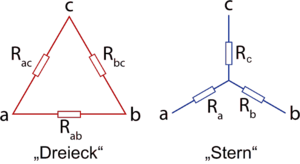
\includegraphics[width=6cm]{bilder/stern-dreieck.png} 
	  \end{minipage}
	  \begin{minipage}[rt]{9.35 cm} %BASTEL!!
      \renewcommand{\arraystretch}{2}
	  \begin{tabular}{ll}
	Umwandlung $\triangle \rightarrow Y$: 
		&$Z_{c} = \dfrac{Z_{ac} Z_{bc}}{Z_{ab}+Z_{bc}+Z_{ac}}$\\
	Umwandlung $Y \rightarrow \triangle$: 
		&$Y_{ac}=\dfrac{Y_{a} Y_{c}}{Y_{a}+Y_{b}+Y_{c}}$\\
	Bei gleichen Widerst\"anden:
	&$R_Y = \frac{R_\triangle}{3}$ \\
	Bei gleichen Kapazit\"aten:
	&$C_Y = C_\triangle \cdot 3 $ \\
	Bei gleichen Induktivit\"aten:
	&$L_Y = \frac{L_\triangle}{3}$
	  \end{tabular}
      \renewcommand{\arraystretch}{1}
	  \end{minipage}
	%\end{figure}
	
	\subsection{Defektleistung von symmetrischen Drehstromverbrauchern}
		\begin{tabular}{| p{7.5cm} | l | l |}
			\hline
 				& Normalleistung		& Defektleistung\\
 			\hline
	 			\textbf{Y-Schaltung bei Leiter- oder Strangausfall} ohne Neutralleiter &
	 				$P_{Norm} = 3 \cdot \frac{U^2_{Str}}{R} = \frac{U^2}{R}$ &
	 				$P_{Def} = \frac{1}{2} \frac{U^2}{R}$ \tiny{nur 50\% von $P_{Norm}$} \\
	 			&&\\
	 			\textbf{Y-Schaltung bei Leiter- oder Strangausfall} mit Neutralleiter &
	 				$P_{Norm} = 3 \cdot \frac{U^2_{Str}}{R} = \frac{U^2}{R}$ &
	 				$P_{Def} = 2 \cdot \frac{U^2_{Str}}{R} = \frac{2}{3} \frac{U^2}{R}$ \tiny{nur 66\% von
	 				$P_{Norm}$} \\ &&\\
	 			\textbf{$\Delta$-Schaltung bei Leiterausfall} &
	 				$P_{Norm} = 3 \cdot \frac{U^2}{R}$ &
	 				$P_{Def} = \frac{U^2}{R} + \frac{U^2}{2R} = \frac{3U^2}{2R}$ \tiny{nur 50\% von $P_{Norm}$} \\
	 			&&\\
	 			\textbf{$\Delta$-Schaltung bei Strangausfall} &
	 				$P_{Norm} = 3 \cdot \frac{U^2}{R}$ &
	 				$P_{Def} = 2 \cdot \frac{U^2}{R}$ \tiny{nur 66\% von $P_{Norm}$} \\
	 		\hline
		 \end{tabular} 
